\documentclass[12pt,a4paper]{article}
%\usepackage[utf8]{inputenc}
%\usepackage[portuguese]{babel}
\usepackage{amsmath, amsfonts, amssymb, mathrsfs}
\usepackage{graphicx}
\usepackage[utf8]{inputenc} % Permite utilizar caracteres especiais: Ex: ç á à...
\usepackage[onehalfspacing]{setspace} % Espaçamento de 1,5
\usepackage{cabecalho}
\usepackage{float}
\usepackage{multirow}
\usepackage[lmargin=3cm, tmargin=3cm, rmargin=2cm, bmargin=2cm]{geometry}
\usepackage{indentfirst}
% \usepackage[brazilian]{babel} % Traduzir para PT-BR
\usepackage{IEEEtrantools}
\usepackage{xcolor}
\usepackage[linesnumbered,ruled,vlined]{algorithm2e}
% Alguns comas
\newcommand{\rxy}{{\mathit{\mathbf{R}}}_{\mathit{x\mathbf{y}}}}
\newcommand{\ry}{{\mathit{\mathbf{R}}}_{\mathit{\mathbf{y}}}}
\newcommand{\wo}{\mathit{\mathbf{w_o}}}
\newcommand{\wn}{\mathit{\mathbf{w}}\left\lbrack n\right\rbrack}
\newcommand{\vn}{\mathit{\mathbf{v}}\left\lbrack n\right\rbrack}
\newcommand{\trans}{\mathsf{T}}
\newcommand{\hermit}{\mathsf{H}}
\newcommand{\mc}[1]{\ensuremath{\mathcal{#1}}}
\newcommand{\mbb}[1]{\ensuremath{\mathbb{#1}}}
\newcommand{\Natural}{\mathbb{N}}
\newcommand{\Integer}{\mathbb{Z}}
\newcommand{\Irrational}{\mathbb{I}}
\newcommand{\Rational}{\mathbb{Q}}
\newcommand{\Real}{\mathbb{R}}
\newcommand{\Complex}{\mathbb{C}}

\newcommand\mycommfont[1]{\footnotesize\ttfamily\textcolor{blue}{#1}}
\SetCommentSty{mycommfont}
\SetKwInput{KwInput}{Input}                % Set the Input
\SetKwInput{KwOutput}{Output}              % set the Output

\begin{document}
	\initcab{Universidade Federal do Ceará}{Inteligência Computacional Aplicada}{Guilherme Barreto}{472525}{Junho/2022}{Neural network - Report}

\section{Work 01 - Rosenblatt's perceptron}

This work considers a classification problem for a multivariate dataset. The iris flower dataset is utilized in a Rosenblatt's perceptron to classify one class from the others. The supervised learning utilizes a common procedure that comprises data preparation, training, test, and analysis of the accuracies for \(N_r\) independent realizations.

The Rosenblatt's perceptron consist in the neuron model architecture, introduced by McCulloch and Pitts in 1943, with a learning algorithm that adjusts the synaptic weights in a supervised fashion. The McCulloch and Pitts' activation function is a step function that triggers the output from 0 to 1 when the induced local field overpass the threshold. This method is effective for binary classification of linearly separable problems, where one can sketch a straight line that divides the classes without overlapping.

At the instant \(n\), the induced local field is given by
\begin{align}
    v(n) = \mathbf{w}^\trans\left(n\right) \mathbf{x}\left(n\right),
    \label{eq:induced-local-field}
\end{align}

where \(\mathbf{w}^\trans\left(n\right) = \begin{bmatrix}
    w_0(n) & w_1(n) & \cdots & w_{N_a}(n)
\end{bmatrix}^\trans\) and \(\mathbf{x}^\trans\left(n\right) = \begin{bmatrix}
    x_0(n) & x_1(n) & \cdots & x_{N_a}(n)
\end{bmatrix}^\trans\) are the synaptic weights of the perceptron and the input signal, respectively, and \(N_a\) indicated the number of attributes. The elements \(w_0(n)\) and \(x_0(n) \triangleq +1\)\footnote{Depending on the author, it can the defined as \(-1\).} are, respectively, the bias and its input.

the machine learning algorithms settles on the well-established theory of adaptive filters. Particularly for the Rosenblatt's perceptron, it is utilized the Least-Mean-Square (LMS) algorithm, that aims to make a instantaneous approximation of the gradient vector. The optimization algorithm is given by
\begin{align}
    \mathbf{w}(n+1) = \mathbf{w}(n) - \eta \mathbf{g}(n),
    \label{eq:w_n+1}
\end{align}
where \(\eta\) is the step-learning hyperparameter and \(\mathbf{g}(n) \triangleq \nabla \mathscr{E} (\mathbf{w})\) is the stochastic approximation of the gradient vector, being \(\mathscr{E} (\mathbf{w})\) the cost function. The \ref{eq:induced-local-field} pass through the step function, \(\varphi \left( \cdot \right)\), generating the perceptron output, \(y\left( n \right) = \varphi(v\left( n \right)) \in \left\{ 0,1 \right\}\). This signal is compared to the desired value, \(d\left( n \right) \in \left\{ 0,1 \right\} \), generating the error signal \(e\left( n \right) = d\left( n \right) - y\left( n \right) \in \left\{ -1, 0, 1 \right\}\), which indicates whether the perceptron misclassified or not. The LMS algorithm uses instantaneous value of the MSE (Mean-Squared Error) cost function, that is,
\begin{align}
    \mathscr{E} (\mathbf{w}) = \frac{1}{2}e^2(n).
\end{align}
Differentiating this equation with respect to the synaptic weights, we get
\begin{align}
    \mathbf{g}(n) = \frac{\partial\mathscr{E} (\mathbf{w})}{\partial \mathbf{w}(n)} = - \mathbf{x}(n) e(n).
    \label{eq:g_n}
\end{align}
Substituting \eqref{eq:g_n} into \eqref{eq:w_n+1}, it yields the learning equation, given by
\begin{align}
    \mathbf{w}(n+1) = \mathbf{w}(n) + \eta \mathbf{x}(n) e(n).
    \label{eq:g_n}
\end{align}

The Algorithm \ref{alg:rosenblatt-perceptron} summarizes the procedure utilized for the Rosenblatt's perceptron, including data preparation techniques, such as hand-out technique and shuffling the dataset. The method utilized \(N_r=20\) independent realization, and pass through the training set \(N_e=100\) epochs. At the end of each realization, it is stored the accuracy reached by the test data, and the results of all accuracies are investigated in terms of mean and standard deviation. The iris dataset contains \(N=150\) instances with \(N_a=4\) attributes (petal length, petal width, sepal length, and sepal width) and \(K=3\) classes (Setosa, Versicolour, and Virginica). It was chosen a ratio of \(80\%-20\%\) for the training and testing dataset, respectively.

\begin{algorithm}[!ht]
    \DontPrintSemicolon
      
      \KwInput{\(\mathbf{X}, \mathbf{D}\) \tcc*{attributes and labels dataset}}
      
    %   \KwData{Testing set $x$}
      \ForAll{\(\left\{ 1, 2, \cdots, N_r \right\}\)}{
        \(\mathbf{w}(n) \leftarrow \text{initialize}\)

        \(\mathbf{X}, \mathbf{D} \leftarrow \text{shuffle}\)

        \( \left( \mathbf{X}_{trn}, \mathbf{D}_{trn} \right), \left( \mathbf{X}_{tst}, \mathbf{D}_{tst} \right)  \leftarrow \text{hold-out}\) \tcc{training and testing dataset}

        \ForAll{\(\left\{ 1, 2, \cdots, N_e \right\} \text{in the training dataset}\)}{
            \(v(n) \leftarrow \mathbf{w}^\trans\left(n\right) \mathbf{x}\left(n\right)\)

            \(y\left( n \right) \leftarrow \varphi(v\left( n \right))\)

            \(\mathbf{w}(n+1) \leftarrow \mathbf{w}(n) + \eta \mathbf{x}(n) e(n)\)

            \(\mathbf{X}_{trn}, \mathbf{D}_{trn} \leftarrow \text{shuffle}\)
        }
        
        \(accuracy \leftarrow \text{test}(\mathbf{X}_{tst}, \mathbf{D}_{tst})\)
      }
    
    \caption{Rosenblatt's perceptron}
    \label{alg:rosenblatt-perceptron}
\end{algorithm}

The process described in Algorithm \ref{alg:rosenblatt-perceptron} was repeated for the classification problem of each class. the Table \ref{tab:rosenblatt-results} shows the results for each class. The setosa classes clearly outperforms the other classes since it is linearly separable for some attributes, as shown in the decision surface in Figure \ref{fig:rosenblatt-decision-surface}\footnote{Since the problem has four attributes, this plot would be impossible as the would get 2 degree of freedom. Therefore, for this result, we considered only these two attributes.}.

\begin{figure}
    \centering
    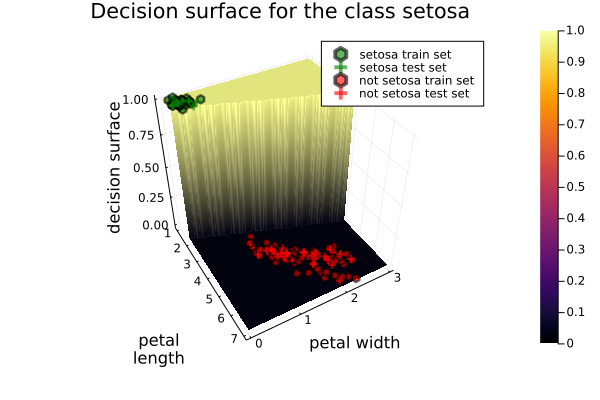
\includegraphics[scale=0.35]{../trab1 (simple perceptron)/figs/decision-surface-for-setosa.png}
    \caption{Decision surface of setosa class.}
    \label{fig:rosenblatt-decision-surface}
\end{figure}

\begin{table}
	\centering
	\caption{Rosenblatt's perceptron performance for classification problem}
	\footnotesize
	\setlength{\tabcolsep}{5pt}
	\begin{tabular}{ccccccccc}
		% \toprule [1.3pt]	
		% \multicolumn{4}{c}{ \textbf{Style} } \\
		\hline
		Classes & mean accuracy & standard deviation \\
		\hline
		Setosa & 98.33 & 0.01972 \\
        \hline
		Virginica & 54.16 & 0.1251 \\
		\hline
		Versicolor & 53.66 & 0.1591 \\
		\hline
	\end{tabular} \label{tab:rosenblatt-results}
\end{table}

The confusion matrix of the setosa class is shown in Figure \ref{fig:confusion-matrix-setosa} for the first realization. The main diagonal indicates that there were not false negative or false positive.

\begin{figure}
    \centering
    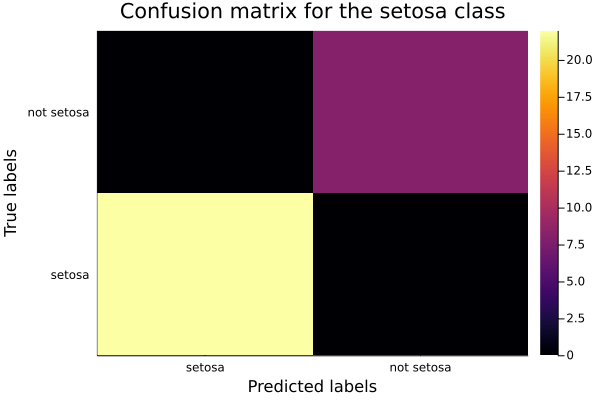
\includegraphics[scale=0.35]{../trab1 (simple perceptron)/figs/setosa-confusion-matrix.png}
    \caption{confusion matrix for setosa class.}
    \label{fig:confusion-matrix-setosa}
\end{figure}

The Figure \ref{fig:setosa-training-evolution} shows the evolution of the training dataset accuracy throughout the epochs. One can notice the fast convergence to accuracy of 100\%.

\begin{figure}[H]
    \centering
    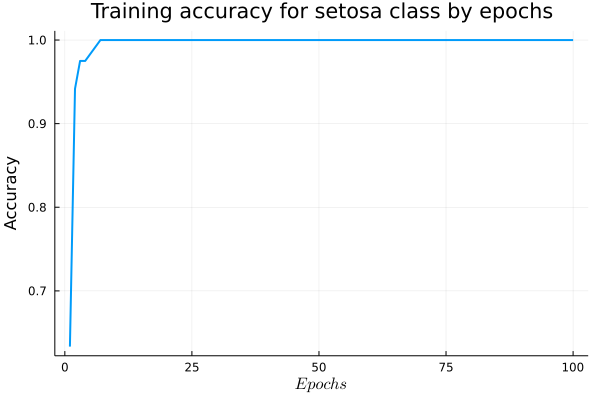
\includegraphics[scale=0.35]{../trab1 (simple perceptron)/figs/accuracy-by-epochs-for-setosa.png}
    \caption{Training dataset evolution for the setosa classification.}
    \label{fig:setosa-training-evolution}
\end{figure}

For a dummy dataset whose the \(K=4\) classes, the Rosenblatt's perceptron achieved a mean accuracy of 97.5\% and a standard deviation of 0.05. The Figure \ref{fig:decision-surface-dummy-data} shows the decision surface of the desired class for the realization whose accuracy the closest to the mean accuracy. All instances of all classes are samples drawn from a Gaussian distribution with a given mean and variance.

\begin{figure}[H]
    \centering
    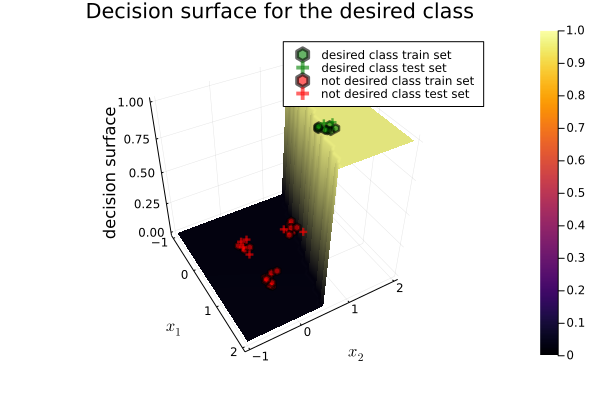
\includegraphics[scale=0.35]{../trab1 (simple perceptron)/figs/decision-surface-for-dummy-data.png}
    \caption{Decision surface for the desired class.}
    \label{fig:decision-surface-dummy-data}
\end{figure}

\section{ADALINE}

The Adaptive Linear Element (or ADALINE) is a variation of the Rosenblatt's perceptron, where the step function is replaced by a linear function, that is, \(y(n) = \varphi(u(n)) = u(u)\). One can combine a tapped delay line with an ADALINE, thus creating an adaptive filter.

Consider a regression problem of adaptive filtering where the input signal is the desired signal corrupted by a Gaussian noise. The ADALINE model tries to retrieved the original data using the same process described in Algorithm \ref{alg:rosenblatt-perceptron}. However, the performance analysis is around the MSE error instead the accuracy since it is now a regression problem.

The Table \ref{tab:adaline-results} shows the performance of the mean MSE and its standard obtained over the independent realizations, in addition the root mean squared error (RMSE).

\begin{table}[H]
	\centering
	\caption{ADALINE performance for regression problem}
	\footnotesize
	\setlength{\tabcolsep}{5pt}
	\begin{tabular}{ccccccccc}
		% \toprule [1.3pt]	
		% \multicolumn{4}{c}{ \textbf{Style} } \\
		\hline
		\(d(n)\) & MSE mean & standard deviation \\
		\hline
		\(ax+b\) & 98.33 & 0.01972 \\
        \hline
		\(ax^2+bx+c\) & 54.16 & 0.1251 \\
		\hline
	\end{tabular} \label{tab:adaline-results}
\end{table}

\end{document}